% xelatex paper
% xelatex paper && bibtex paper && xelatex paper && xelatex paper

\documentclass{nime-alternate} % Uncomment when publishing final version

% Uncomment only one of the ones below
% \usepackage{anonymize} 		   %Uncomment this line to publish
\usepackage[blind]{anonymize}%Uncomment this line for blind review

\usepackage[utf8]{inputenc}

\usepackage{stfloats}
\usepackage{amsmath}

\begin{document}

% --- Author Metadata here ---
\conferenceinfo{NIME'24,}{4--6 September, Utrecht, The Netherlands.}

\title{Malletwand: the Pendulum as a Handheld Interface to Musical Timing}

\label{key}
\numberofauthors{4}
\author{
\alignauthor
\anonymize{Lyu, S.} \\
  \affaddr{\anonymize{Academy of Arts \& Design, Tsinghua University}}\\
  \affaddr{\anonymize{Beijing, China}}\\
  \email{\anonymize{claire@ayu.land}}
\alignauthor
\anonymize{Li, H.} \\
  \affaddr{\anonymize{Academy of Arts \& Design, Tsinghua University}}\\
  \affaddr{\anonymize{Beijing, China}}\\
  \email{\anonymize{lihanxua22@mails.tsinghua.edu.cn}}
\and
\alignauthor
\anonymize{Wang, R.} \\
  \affaddr{\anonymize{Academy of Arts \& Design, Tsinghua University}}\\
  \affaddr{\anonymize{Beijing, China}}\\
  \email{\anonymize{wangrh22@mails.tsinghua.edu.cn}}
\alignauthor
\anonymize{Mi, H.}\titlenote{Corresponding author.}\\
  \affaddr{\anonymize{Academy of Arts \& Design, Tsinghua University}}\\
  \affaddr{\anonymize{Beijing, China}}\\
  \email{\anonymize{mhp@tsinghua.edu.cn}}
}
\date{6 February 2024}

\maketitle

\begin{figure*}[h!]
  \centering
  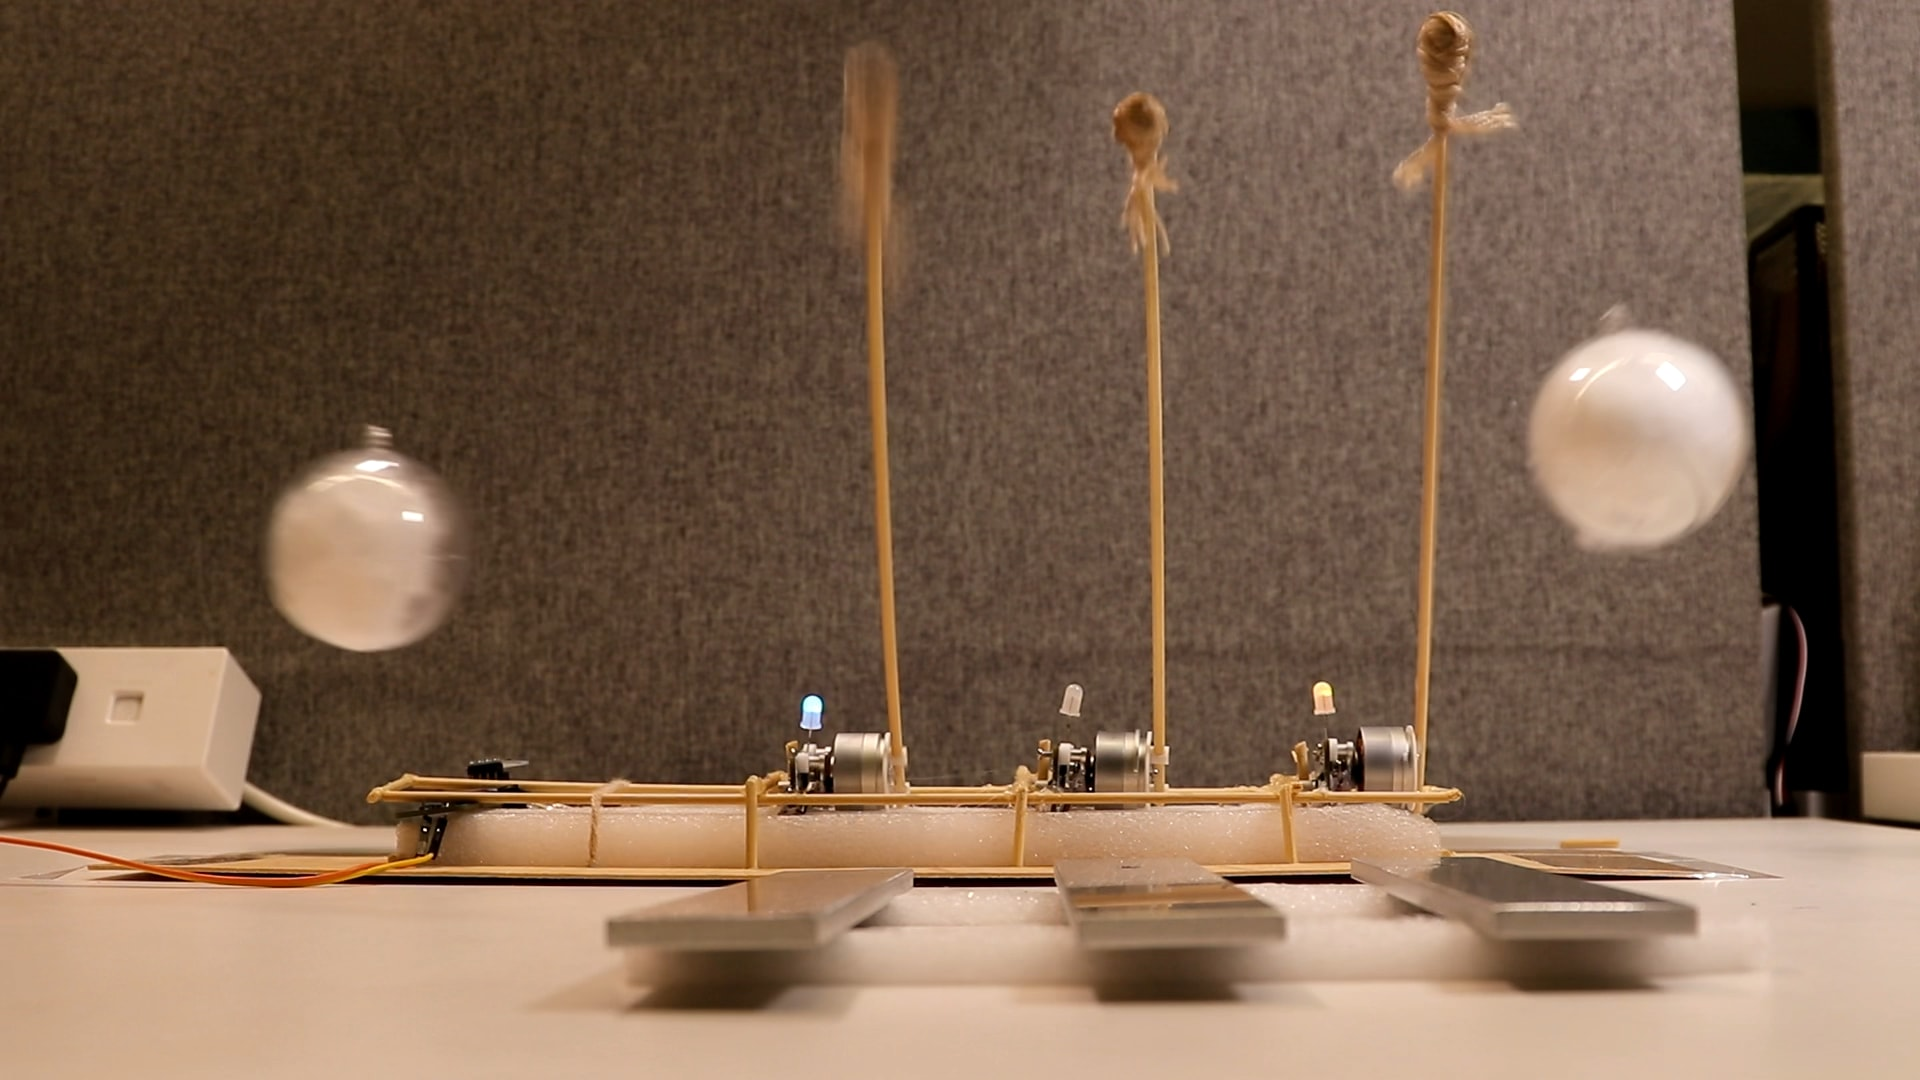
\includegraphics[width=1\textwidth]{Mw_Banner.jpg}
  \caption{The Malletwand controllers with the prototype self-playing glockenspiel.}
  \label{fig:Banner}
\end{figure*}

\begin{abstract}
We devise and implement an interface in the form of a handheld pendulum device for manipulating the timing of musical playback. The physical properties of the pendulum make this interaction scheme steady and intuitive, and particularly suitable as an introductory means of musical engagement for untrained participants. We build a self-playing glockenspiel around this interface to demonstrate how our design encourages musical exploration and social play. We conclude by discussing potential extrapolations and integrations of the design in mobile and hybrid scenarios.
\end{abstract}
\keywords{Musical interface, pendulums, tactility, pose estimation, HCI}

\ccsdesc[500]{Applied computing~Sound and music computing}
\ccsdesc[300]{Human-centered computing~Interaction devices}
\ccsdesc[300]{Hardware~Sensor applications and deployments}
\printccsdesc


\section{Introduction}

Throughout our experience, we have always been able to capture the instinctive desire to actively and earnestly engage in music from those that have not had the advantage to experience music full-scale (pun intended).
In our lasting endeavour to expand the reach of musically-meaningful interactive experiences, we set out on a search of an interaction scheme that is easy to understand and operate without musical expertise, while navigating the participant in sensible directions to manipulate the sounds to their own imagination, deepening their connection with the musical elements they have been presented with.

We settled on the periodic motion of the pendulum. The stability and self-recovering property of pendular motion makes for a reliable framework of periodic musical time, i.e., tempo, or beats.

We devise and implement a controller interface, which we title the Malletwand, in the form of a handheld pendulum device. By swinging the pendulum, the participant is able to manipulate the speed of musical time, while the kinematic properties gently guides them through its tendency to keep a stable period, preventing excessive deviance from a steady tempo.

We imagine that this interface be paired with various types of musical actuators. For this report, we build a self-playing glockenspiel (the ``mallet'' in the name) operated by up to two such controllers in order to demonstrate how our design encourages musical exploration and social play.

The rest of the article is outlined as follows. We provide an overview of related work in various relevant fields before presenting the details of our design and implementation of the controller interface and the self-playing instrument. We go on to discuss potential extrapolations and integrations of the design in mobile and hybrid scenarios, some of which we plan as our future work. Algorithmic details are laid out in the appendix.

\section{Related work}

As we direct our design towards approachability for all levels of expertise, we look for intuitive universalities among human music, and directed our attention to the formation and perception of isochronal patterns based on the abundant argument that humans naturally tend to perceive time, and especially in the musical context, in cycles and patterns~\cite{Brower:Cog, Neisser_1976, Ravignani2016}. To paraphrase our forerunners, repeating cycles of time set the boundaries of our activities as well as form grounds on which we anticipate our sensory stimuli. Discussions went further to establish the metaphorical and cognitive interplay our sense of time with embodied motion~\cite{Johnson_Larson_2003, Johnson_2008}.

Indeed, there have been a number of devices that manifest the link between periodic bodily movement and stable temporal patterns. Scrubbing is a standard technique for turntablists to manipulate the speed of sounds by rotating vinyl records. Hand-cranked musical boxes provide a more approachable way to drive the flow of music by one's own hands; although the Swedish band Wintergatan went as far as to build an entire machine, the Marble Machine, that turns the revolution of the manual crank into the progression of a musical piece~\cite{Rundle_Woollaston-Webber_2017}.

However, these devices share the common limitation that they require practice, or at least familarity with steady bodily movement, to prevent sounds from being distorted in the temporal domain. Laypeople tend to invoke unsteady musical time on such devices, rendering the music less understandable and aesthetically pleasing, while it remains unclear to them how they should refine their actions in the reasonable directions. Thus, they will not be able to get the most out of the tactile musical experience.

From another perspective, we are delighted to see novel musical devices that employ pendular motion or handheld physical controllers. Kugelschwung~\cite{Kugelschwung} is a digital musical instrument that relies on a set of pendulums mounted on a tabletop frame supplying control signals for soundscapes. Le Bâton~\cite{LeBaton} maps the chaotic behaviour of the triple pendulum into unpredictably varying electronic sounds. Gyrotyre~\cite{Gyrotyre}, on the other hand (no pun intended), is a handheld controller that maps oscillating signals from a gyroscope on a precessing wheel to various musical applications.

Still, these interfaces and instruments take larger physical forms and mainly aim at stage performances and/or dedicated experimental production setups. Our design adds to this ensemble a missing piece: a lightweight handheld controller interface that can be enjoyable and meaningful regardless of the participant's prior musical experience.

\section{The ``Wand''}

\subsection{Design Overview}
We first present the details of the handheld controller interface. It takes the form of a handle with a hanging bob (ball) that can freely swing and spin around, forming a pendulum. The participant swings the pendulum at their desired frequency while the bob's quasi-periodic motion is mapped to continuous musical time such that each fastest-moving point in a period corresponds to the start of a beat. (This point is usually perceived to be the ``central'' or the ``lowest'' point in simple pendulums, but since our pendulum has an extra degree of freedom, i.e., is a spherical pendulum, this appointment needs to be extrapolated.) Such generated timing signals are wirelessly transmitted to an actuator (instrument) that plays a piece of music according to the manipulated flow of musical time.

We add a few simple features to enrich the feedback and interaction. Haptic feedback at beat onsets is provided by a vibration motor. A tri-colour LED is placed inside the bob that is flexible in its responses to interaction, e.g., it may indicate the changing beats by alternating tints or identify the voice by colour coding in the case of multiplayer interaction. Furthermore, the controller is intended to be normally at rest, so it is equipped with a vibration switch that wakes up the entire circuit from sleep when the device is picked up by a participant. A single-pole, single-throw (SPST) switch allows the overall power to be turned off during times without participants.

\subsection{Construction}
We design customised electronics for all of our devices. The handle contains a lithium polymer (Li-Po) battery, a microcontroller, a radio transceiver, a vibration motor, and various supporting components; the bob contains MEMS chips that form a 9-axis IMU (an accelerometer, a gyroscope, and a geomagnetometer). The complete structure is illustrated in Figure~\ref{fig:WandConstruction}.

\begin{figure*}[t!]
  \centering
  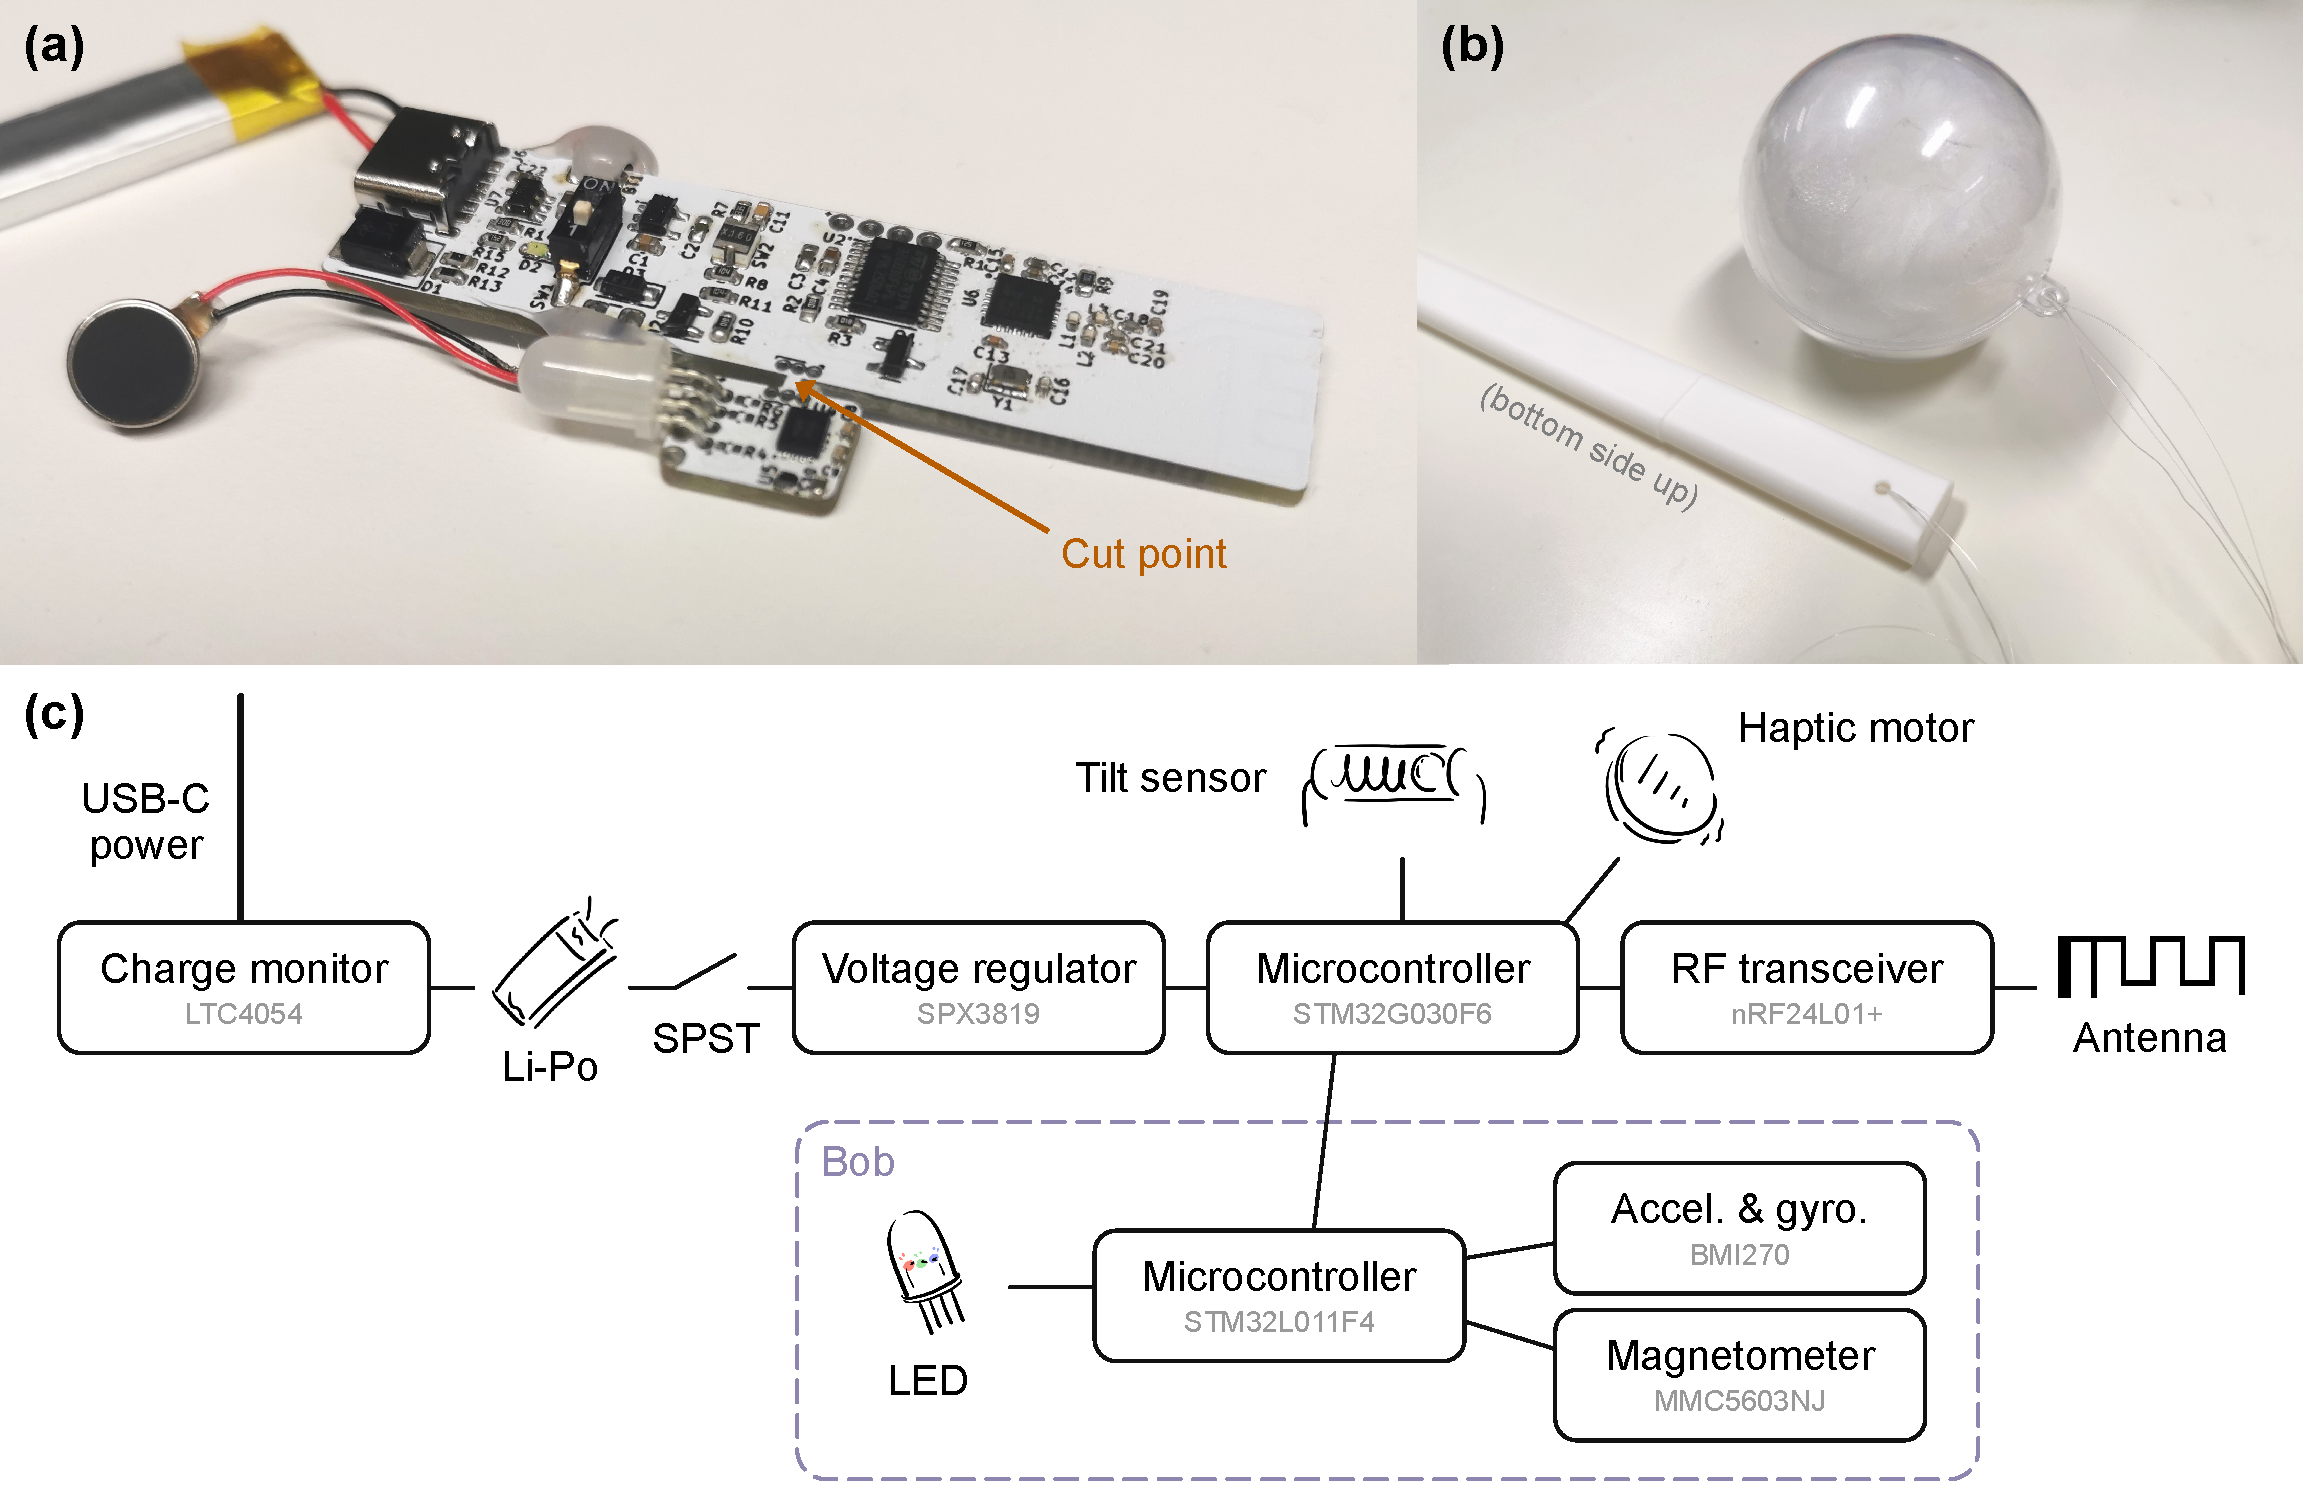
\includegraphics[width=1\textwidth]{Mw_Wand.pdf}
  \caption{(a) Photo of the assembled circuit board before being cut. (b) Block diagram of the electronic components involved.}
  \label{fig:WandConstruction}
\end{figure*}

The board is fabricated as one, in order to ease soldering and debugging as we build the prototype. After testing is complete, we cut the board at the thin connection (in Figure~\ref{fig:WandConstruction}a) and connect the two parts with thin wires (8 strands of 32 AWG). The handle part is glued inside a 3D-printed casing with the wires hanging down onto the bob part, which is inserted onto a holder made of polymeric foam glued in a translucent plastic sphere filled with down cotton. We add fishing wires to strengthen the connection and prevent the electric wires from excessive tension and fatigue.

\subsection{Estimation Algorithm}
All processing is done on the microcontroller device. The microcontroller we used, STM32G031, is an Arm Cortex-M0+ processor without a dedicated FPU, but our complete algorithm runs well within its 64 MHz system clock with software floating-point arithmetic.

The algorithm requires an initial orientation calibration before employing an ensemble of filters to process the sensor signals. The calibration step is run once after assembly and before finishing deployment. We introduce these two parts respectively. To keep our description concise, we defer all of the mathematical details to Appendix~\ref{appendix:signal-processing}.

\subsubsection{Orientation calibration}
After assembly, the orientation of the circuit board inside the bob should be compensated for.

The calibration is triggered by a wireless radio signal. The operator is then expected to hold the handle and let the bob stay stationary for a short while. Signals from the accelerometer are continuously monitored until they reach a sufficiently low deviation throughout a fixed time window of 3 seconds. This yields an axis vector that acts as the reference for future motion estimation from sensor readings which is saved in the persistent flash storage of the microcontroller. For details, please refer to Appendix~\ref{appendix:calib-ori}.

\subsubsection{Magnetometer calibration}
As our algorithm relies on the geomagnetometer to improve accuracy of pose estimation, the distortion of the ambient magnetic field should also be compensated. Since indoor environments contain prominent and variable magnetic interference, this calibration is done online during operation. This works by continuously collecting the readings of the magnetometer and finding an ellipsoid fit that tries to distort the collected data in the form of 3D vectors onto a unit sphere. We employ the adjusted least squares estimator introduced by \cite{Markovsky_2004_ALS} with complementary steps by \cite{Renaudin2010}.

\subsubsection{Motion signal processing}
Our IMU produces readings at a sampling rate of 100 Hz, and the filtering algorithms run at the same rate. At each time step, we first estimate the facing of the bob through a complementary filter, inspired by~\cite{Min_Complementary}, combining signals from the gyroscope and the magnetometer. The result is turned into a rotational transform that cancels out the bob's rotation around its own axis. Sensor readings adjusted by this transform are then fed into an extended Kalman filter (EKF) that estimates the trajectory of the bob in 3D space, and more importantly, its current phase within the period of motion. This is the value that gets interpreted as the driving signal of musical time, and is transmitted to the actuator.

Also transmitted is a confidence indicator, which is the Frobenius norm of the estimation covariance matrix in the EKF. This value allows both the controller and the actuator to avoid muddled time progression when the motion is not stably periodic, e.g., during the first few seconds since the beginning of interaction.

\section{The ``Mallets''}

\subsection{Design Overview}
Our demonstrative self-playing instrument is a 21-key glockenspiel that spans a register of 2.3 octaves by the diatonic major scale with the raised fourth and the flat sixth added.

The instrument is accompanied by two Malletwand controllers and can operate in both solo and co-operative mode. Signals received from the controllers drive the passing of musical time in a predetermined musical piece, similar to a musical box. Co-operative mode is entered by two controllers being operated simultaneously, where each controller corresponds to one voice (part) indicated by colours of the lights. The music only progresses when the motion of the two are roughly in synchronisation.

\subsection{Construction}
\subsubsection{Keys}
The keys are laser-cut from aluminum of 5 mm thickness. We chose aluminum instead of an alloy since we would like a mellower timbre. Prior to production, we ordered a small number of samples from the fabricator to determine the acoustic characteristics of the material, i.e., timbre and the coefficient for resonant frequency. The resonant frequency of a vibrating metal bar is inversely proportional to the square root of its length. We thus calculate the desired lengths according to equal-temperament tuning, create the blueprints programmatically in OpenSCAD and send them for fabrication.

\begin{figure*}[t!]
  \centering
  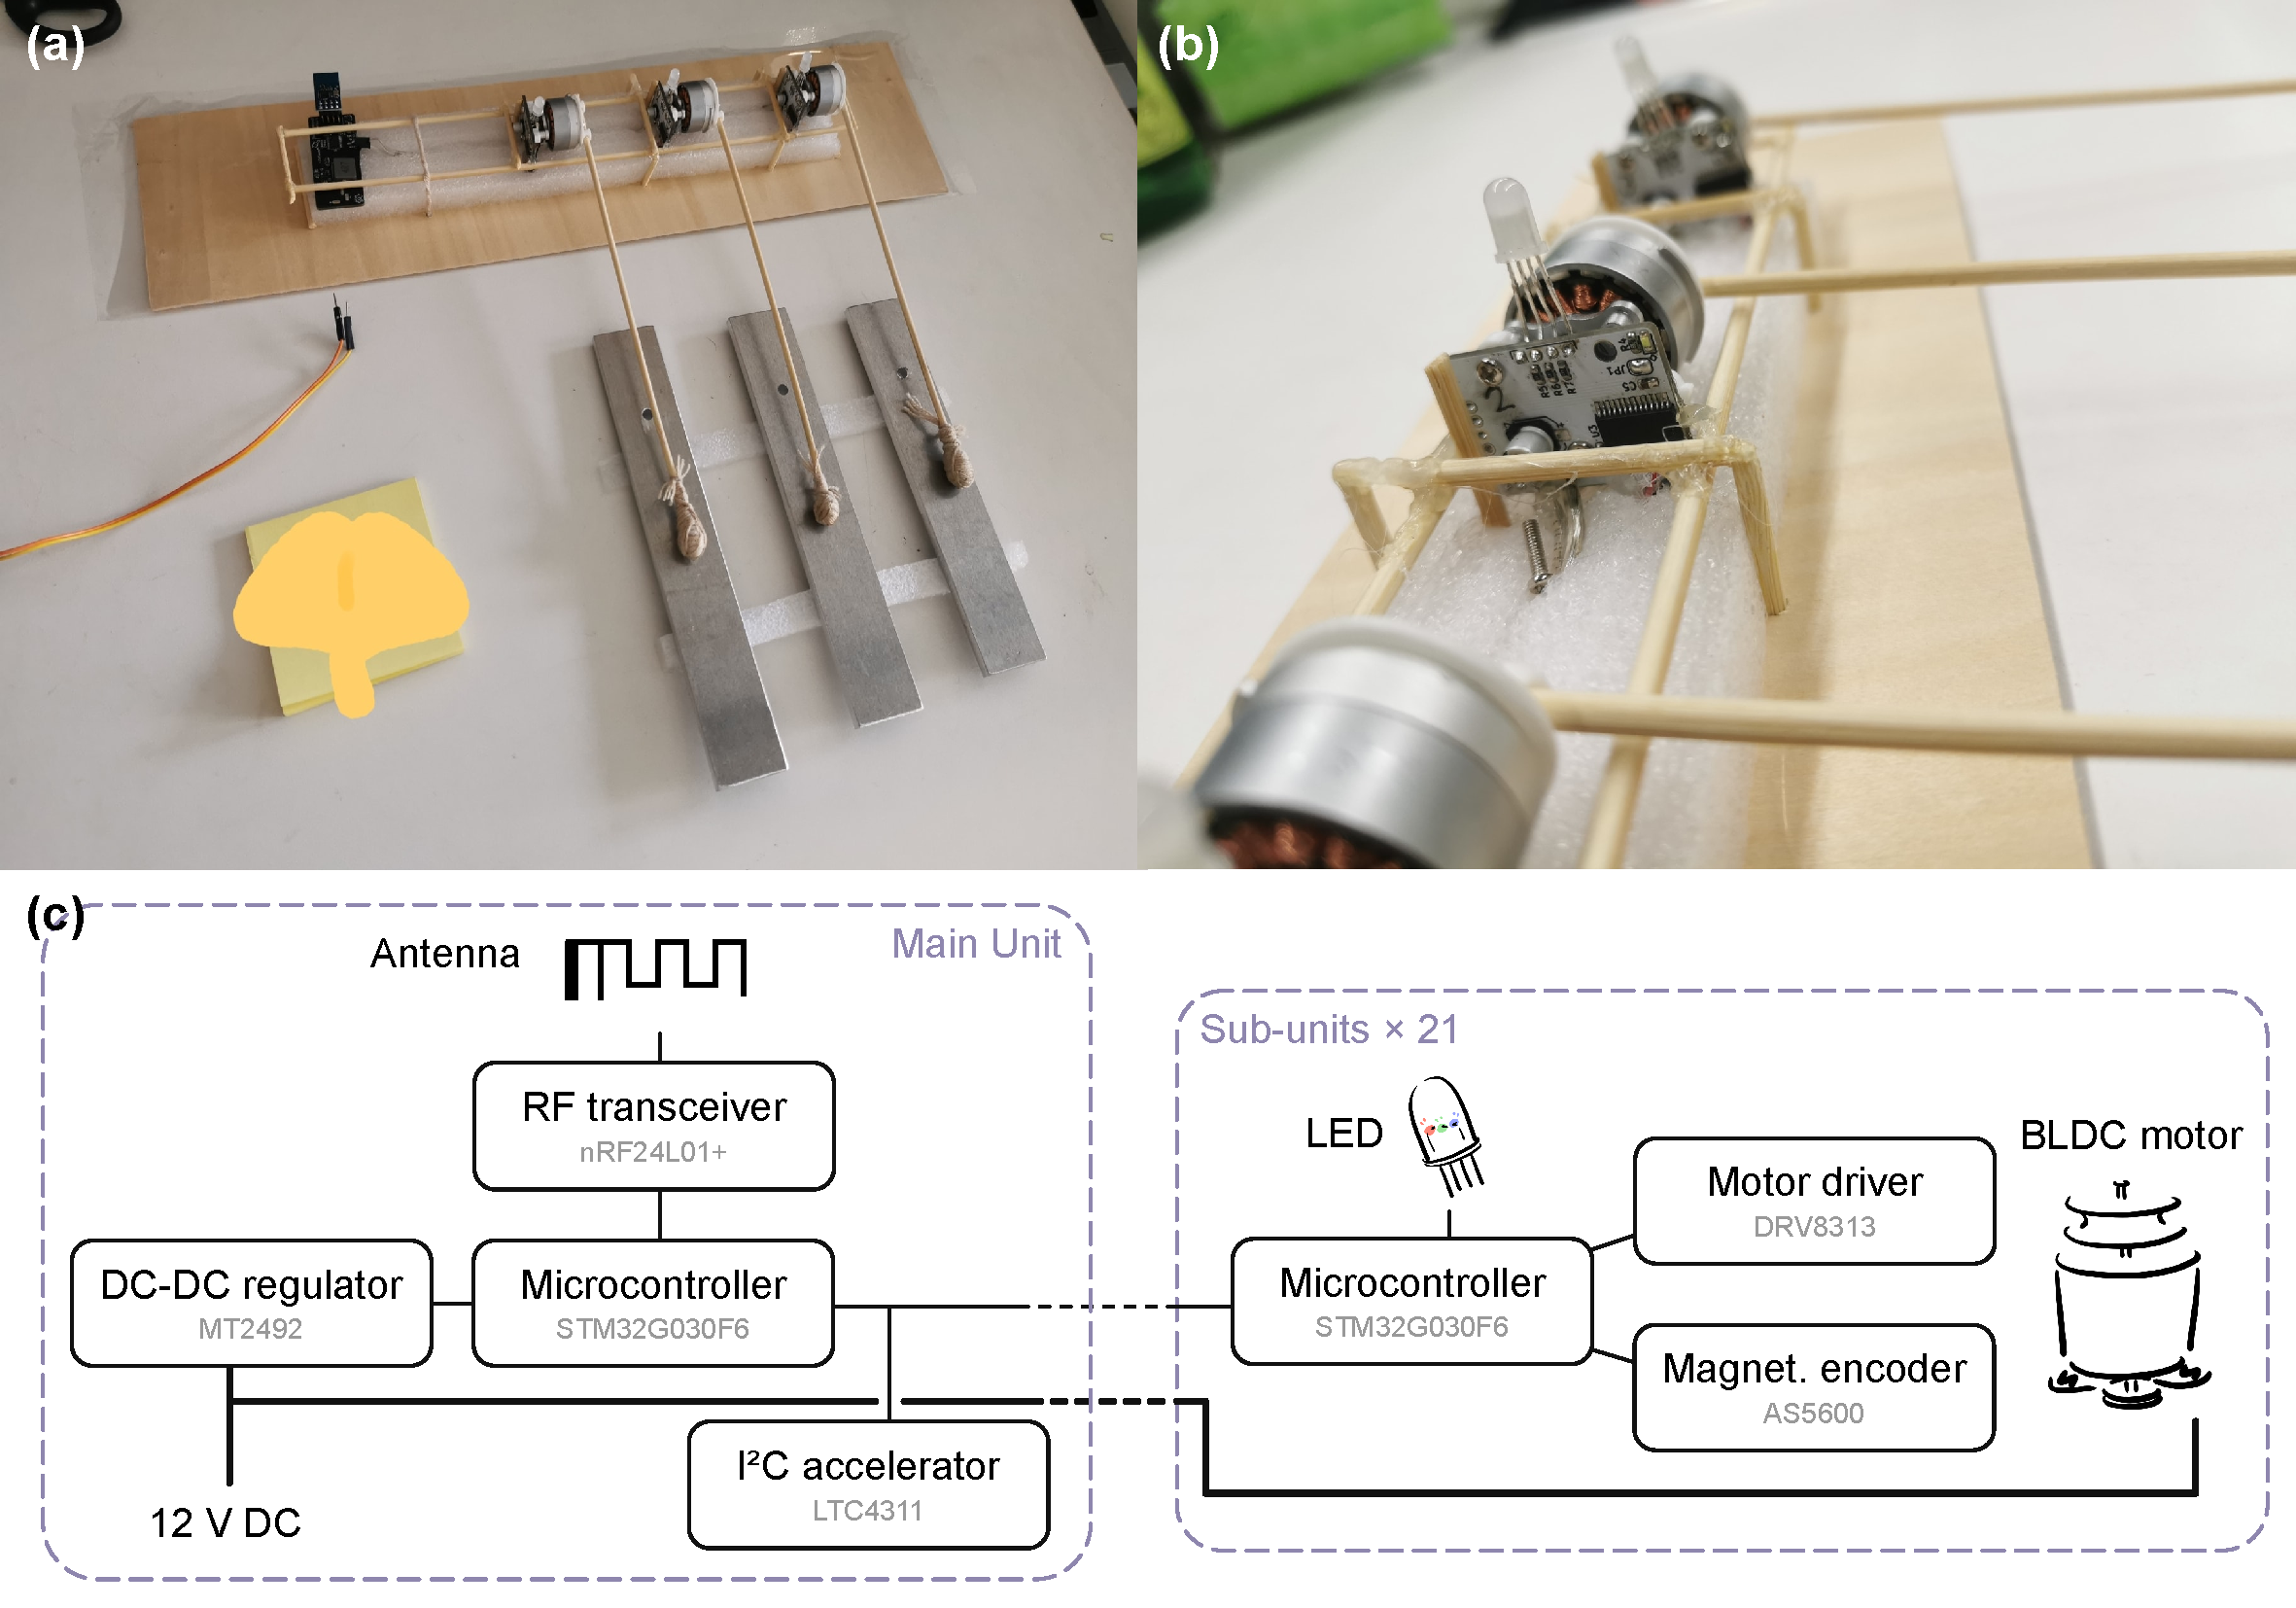
\includegraphics[width=1\textwidth]{Mw_Mallet.pdf}
  \caption{(a) Overall photo of the instrument. (b) Close-up of a single sub-unit. (c) Block diagram of the electronic components involved.}
  \label{fig:MalletConstruction}
\end{figure*}

\subsubsection{Electronics}
The electronics of the instrument comprise a main unit and 21 sub-units~\footnote{We have not finished assembling all the keys as of the time of submission of this manuscript; we hence temporarily use our 3-key prototype for demonstrations.}, one for each key. The main unit is responsible for the communication with the controller(s) as well as the delivery of power and control signals to the sub-units. Each sub-unit has a small BLDC motor that holds a yarn mallet, fixed onto a circuit board with a magnetic encoder, a tri-colour LED, and a microcontroller. The entire device is powered by a single DC supply between 9 V and 25 V into the main unit. The complete structure is illustrated in Figure~\ref{fig:MalletConstruction}.

We choose I\textsuperscript{2}C as the communication protocol, because it needs only two electrical signals for multiple parallel devices. We use an I\textsuperscript{2}C accelerator chip on the main unit to get around rise time issues due to increased bus capacitance of long transmission wires.

\subsubsection{Mechanical and miscellaneous}
We fix all units (both the main one and sub-units) onto polymeric foam which is glued onto a thin wooden board that serves as the base. Slots created on the foam hold the units as well as the electrical lines. We glue an extra frame made of wooden sticks around the foam to improve stability.

The mechanical parts for the fixation of motors and mallets are all 3D-printed with PLA. Yarn on the mallets are manually wrapped around a wooden core and slightly melted with a lighter in order to tighten it.

\subsection{Performance}
During operation, the glockenspiel plays a tune as the pendulum(s) swing(s) back and forth. The tempo of the music adjusts to the period(s) of pendular motion. Haptic feedback and lights on both the bob and the keys add tactility and visualisation to the embodied musical experience. Figure~\ref{fig:Banner} is a photo of the instrument in action.

Please refer to the attached video for a performance recording.~\footnote{The video is available at \url{http://bit.ly/42xa08Q} during review. We have removed traces of the authors' identities.}

\section{Discussion}

\subsection{The Experience of Malletwand}
Our design accomplished our initial goals. The algorithms yield a reliable estimation of motion, successfully running the glockenspiel through a tune steadily with little external intervention on the pendulum, while being able to respond reasonably fast to changes in motion (within 1\textasciitilde{}2 swings). We enjoyed our own work.

Through our pilot study, we confirmed that the pendulum-based interface is appreciated for its accuracy and ease of use. First-time users might not instantly figure out how to reliably manipulate the speed (period) of the pendulum, but were able to do so with their own exploration or with a hint. Since participants were able to quickly grasp the control and the mapping logic, musical exploration was instantly opened up to them. Participants tended to experiment with extremes before resorting to a steady tempo, trying gentler articulations, and were generally successful in their pursuit of musical expression.

Social play is encouraged through the attempts to synchronise between the duo. This resembles the experience of musicians in ensembles, orchestras, or bands, and is appreciated by such practitioners. However, we notice that this is a rare and precious chance for participants with less musical experiences, and we hope to bring such meaningful and joyful activities to their reach through our design. We are still yet to conduct more extensive studies with such participants.

One major shortcoming of the co-operative mode is the difficulty to synchronise the phases between the duo, due to inertia preventing quick changes in speed, even more so regarding phase and position. This has the benefit of extending conversations between participants, but the less experienced of them might not figure out effective ways quickly and intuitively. In this regard, we are considering improving on the co-operative play mode, either by revamping the interaction rules or by extra hints in the form of synchronised haptic feedback or textual hints.

\subsection{Extrapolations and Future Work}
As we have written in the Introduction section, we imagine that this interface not be limited to our glockenspiel instrument. Any device that plays music can employ a pendulum interface to invite participants into musical time. Hybrid formats, including projections and mappings, or musical devices remotely incited beyond kilometers, opens doors to tactility in a hybrid world.

Other musical features, or even other temporal formats, or even spatial expositions, may be involved as well. What about an installation that gives procedurally generated sounds? What about a film? A dance? A video game where cats chase the wand? A kaleidoscope? A planetarium?

The estimation algorithms in the pendulum enable it to act as a standalone sensor, adding to the toolkit of digital artistic expression. What about an electronic mimicry of a windbell? A big hanging simulated telescope? A sparkling earring?

Another possible extrapolation lies in the mobile scenario. The sensors we used are standard in today's smartphones, and relevant APIs are readily available on modern web browsers. Thus, with the processing algorithms ported to JavaScript, websites will be able to create novel interactive experiences without special equipment, simply by asking the visitor to put their phone in a holder, attach a string, and swing it to their liking. What about such a musical box? We leave all these for the reader as exercises while we try our hands on a few.

\section{Conclusion}
Malletwand is our first step in spreading the enjoyablility of music through a tactile medium. It is to our delight to have implemented the system and seeing it bear the unique approachability and adaptability to varied levels of musical expertise, adding to the state-of-the-art (pun intended) repertoire of physical-system controller interfaces. We realise that this interface has the potential to adapt to more instruments and scenarios, and put forward what we have envisaged. We share our work in the hope that our methods and insights can be useful to those who share the aspirations with us.

\section{Acknowledgments}
Anonymised.

\bibliographystyle{abbrv}
\bibliography{nime-references} 

\appendix
\section{Details of the Signal Processing Algorithms}
\label{appendix:signal-processing}
We try to outline the mathematical derivations of the algorithms. For details, please refer to the source code.

\subsection{Calibration}
\subsubsection{Orientation}
\label{appendix:calib-ori}
An accelerometer reading is a 3-dimensional vector. When a sufficiently low variation of readings is achieved during calibration, their average vector is normalized and taken as the reference axis $\mathbf{u}$. We find a quaternion $\mathbf{q}$ that rotates this vector to the $+z$ unit vector, $\mathbf{z}^+ = \begin{bmatrix} 0 & 0 & 1 \end{bmatrix}^\mathsf{T}$. This is achieved by setting $\mathbf{q}_1 = \begin{bmatrix} \mathbf{u} \times \mathbf{z^+} & (1 + \mathbf{u} \cdot \mathbf{z^+}) \end{bmatrix}$ and $\mathbf{q} = \mathbf{q}_1 \mathbin{\mathop{/}} \lvert \mathbf{q}_1 \rvert$.

This quaternion $\mathbf{q}$ transforms the reference frame of the accelerometer such that the $xy$ plane corresponds to the local ground, whose normal vector is the $z$ axis. The rotation specified by $\mathbf{q}$ is applied to future raw accelerometer readings $\tilde{\mathbf{a}}$ and gyroscope readings $\tilde{\mathbf{g}}$, assuming that their reference frames are aligned, to yield a carlibrated 6-axis reading: % , as well as the magnetometer readings after its own calibration has been carried out, in order to give an absolute orientation with reference to the ground (refer to the explanation below for further details).
\begin{equation}\label{eqn:calib-ori}
\begin{aligned}
\mathbf{a} &= \mathbf{q} \tilde{\mathbf{a}} \mathbf{q}^{-1}\text{,} \\
\mathbf{g} &= \mathbf{q} \tilde{\mathbf{g}} \mathbf{q}^{-1}\text{.} \\
\end{aligned}
\end{equation}

\subsubsection{Magnetometer}
\label{appendix:calib-mag}
This task can be formulated as follows: given a set of 3-dimensional vectors $\{ \tilde{\mathbf{m}}_i \}$, find an affine transform $(\mathbf{Q}, \mathbf{o})$ such that the set of $\{\mathbf{Q} \tilde{\mathbf{m}}_i + \mathbf{o}\}$ best fits onto a unit sphere.

We follow the method of \cite{Renaudin2010}, employing the ALS estimator in \cite{Markovsky_2004_ALS} to find a fit $(\mathbf{A}, \mathbf{c})$ to the set of equations
$(\tilde{\mathbf{m}}_i - \mathbf{c})^\mathsf{T} \mathbf{A} (\tilde{\mathbf{m}}_i - \mathbf{c}) = 1$
and then calculating an inverse transform that converts this ellipsoid back to the unit sphere.

Since the ALS estimator only requires an accumulated matrix $\mathbf{\Psi}$ and not the individual $\tilde{\mathbf{m}}_i$, we are able to carry out the calculation online in constant rather than linear memory space.

\subsection{Estimation}
\subsubsection{Facing}
\label{appendix:est-facing}
Our complementary filter design follows that in~\cite{Min_Complementary}, namely, one satisfying the transfer equation
\begin{equation}
\begin{split}
& \hat{\theta} = \frac 1 {s^2 + k_\mathrm{p} s + k_\mathrm{i}} \left( s \dot\theta + (k_\mathrm{p} s + k_\mathrm{i}) \theta \right) \text{,} \\
& k_\mathrm{p} = \frac {\omega_0} {Q_\mathrm{P}},\qquad k_\mathrm{i} = \omega_0^2\text{.}
\end{split}
\end{equation}
This filter balances between a proportional signal $\theta$ and a derivative signal $\dot\theta$. Here we treat the 2-dimensional orientation on the $xy$ plane as the value being estimated. The calibrated magnetometer provides the $\theta$ signal, while the calibrated gyroscope provides $\dot\theta$.

The input signals are given by $\theta = -\mathop{\mathrm{arctan}} \frac {\mathbf{m}_y} {\mathbf{m}_x}$ and $\dot\theta = \mathrm{d}{\mathbf{g}_y} \mathbin{\mathop{/}} \mathrm{d}t$. Here $\mathbf{m}$ is the calibrated and aligned magnetometer reading,
\begin{equation}\label{eqn:est-facing}
\mathbf{m} = \mathbf{q} \ (\mathbf{Q}\tilde{\mathbf{m}} + \mathbf{o}) \ \mathbf{q}^{-1}\text{.}
\end{equation}
% , and $\mathbf{g}$ is the calibrated gyroscope reading $\mathbf{g} = \mathbf{q} \tilde{\mathbf{g}} \mathbf{q}^{-1}$.

We fix the pole quality factor as $Q_\mathrm{P} = 1 \mathbin{\mathop{/}} \sqrt{2}$ and manually and empirically tune the corner frequency at $\omega_0 = 24\ \text{rad/s} \approx 3.8\ \text{Hz}$. A slightly different value might be needed if the characteristics (models) of sensors change.

\subsubsection{Motion}
\label{appendix:est-motion}
In the extended Kalman filter we formulate the state vector as $\mathbf{x} = \begin{bmatrix} \omega & A & \theta & B & \phi \end{bmatrix}^\mathsf{T}$, where the observation $\mathbf{z} = \begin{bmatrix} A \cos \theta & B \cos (\theta + \phi) \end{bmatrix}^\mathsf{T}$ is the gyroscope readings adjusted by the facing estimation,
\begin{equation}
\begin{split}
\hat{\mathbf{g}}' &= \mathbf{r}_{z, \theta} \hat{\mathbf{g}} \mathbf{r}_{z, \theta}^{-1} \\
\mathbf{r}_{z, \theta} &= \begin{bmatrix} 0 & 0 & \sin \frac \theta 2 & \cos \frac \theta 2 \end{bmatrix}
\text{,}
\end{split}
\end{equation}
projected onto the $xy$ plane. Varying $\theta$ over $[0, 2\pi)$ traces out an elliptic trajectory of this point and $\theta$ is the current phase within the period. $\omega$ is the rate of increment of $\theta$.

The prediction function is
\begin{equation}
f(\mathbf{x}) = \begin{bmatrix} \omega & A & \theta + \omega \Delta t & B & \phi \end{bmatrix}^\mathsf{T}\text{.}
\end{equation}
The process noise covariance matrix is set to be a diagonal matrix with the first entry prominently larger than the others, since $\omega$ is actively changed by the participant. If $A, \theta, B, \phi$ are assigned large process noise variances, the filter may frequently get stuck in a local optimum where all parameters oscillate, altogether stopping the steady progress of phase.

After the estimation of $A, \theta, B, \phi$ are obtained, we find the tilt angle of the major axis by $\delta = \frac 1 2 \mathop{\mathrm{arctan}} \frac {A^2 + B^2 \cos 2\phi} {B^2 \sin 2\phi}$, and calculate the difference $\theta - (\delta + \frac 1 4 \pi)$ to align the zero phase to the fastest-moving point.

\section{Source Repository}
All of our design files (printed circuit board assemblies, mechanical models) and source code are published at \newline \anonymize{\texttt{https://github.com/ayuusweetfish/Malletwand}}.

\end{document}
